Once our results were verified to be correct, we ran the simulation on
RPI's BG/Q supercomputer, AMOS, in order to quantify the benefits
obtained through parallelization. Execution time was measured using a
high-precision cycle counter, implemented in the simulation by Kevin
O'Neill. Subsequent runs for analysis were then conducted and logged
on AMOS by Mitchell Mellone.

\subsection*{Strong Scaling Study}
\begin{figure}[h!]
  \centering
  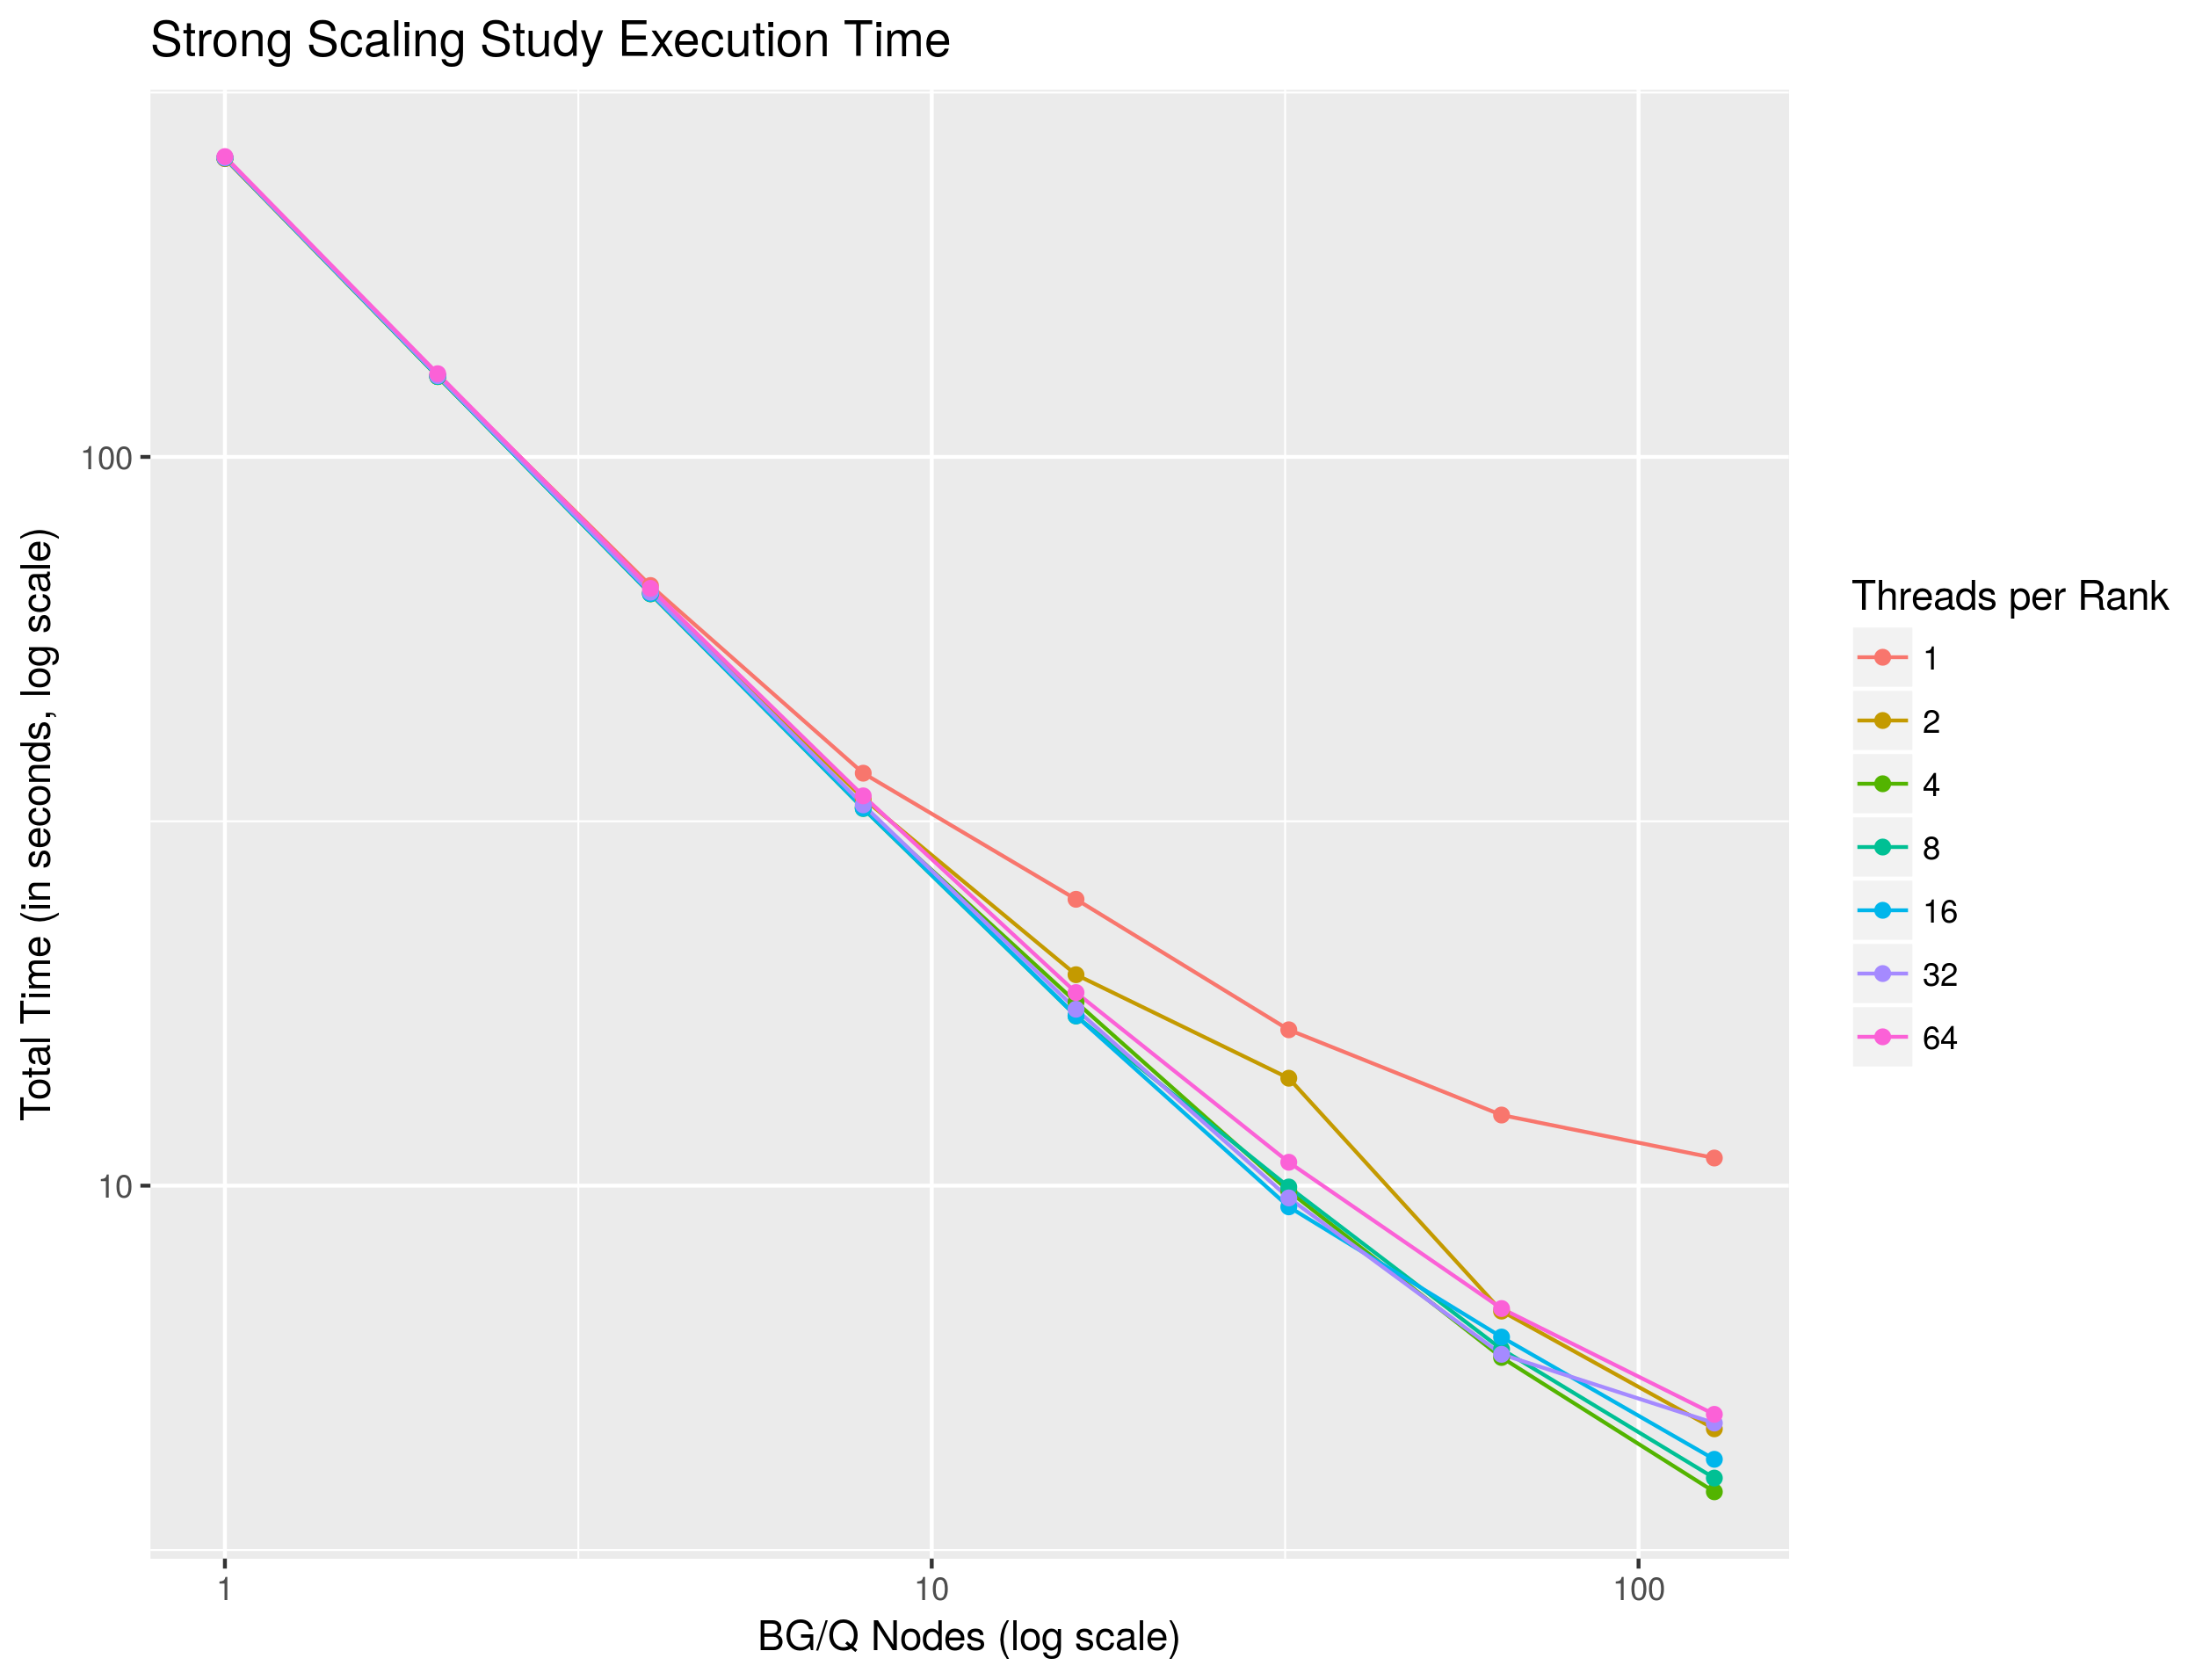
\includegraphics[width=\linewidth]{total_time.pdf}
  \caption{Execution time for 8192 birds and 1000 iterations.\label{fig:total}}
\end{figure}

The plot in Figure \ref{fig:total} shows the results of our strong
scaling study which measured the execution time required to simulate
8192 birds for 1000 iterations, using 1, 2, 4, 8, 16, 32, 64, and 128
BG/Q nodes. Each BG/Q node has a 16 core processor with 4-way
multithreading per core, therefore we ran a combination of 64 MPI
ranks * pthreads per node ranging from 64 MPI ranks with one pthread
per rank to one MPI rank with 64 pthreads per rank. We can see that
this simulation scales fairly well from 64 to 512 ranks * pthreads
(one to eight BG/Q nodes). As we continue to scale up we start to see
much more pronounced performance differences between the different
thread per rank configurations. In particular, using only one thread
per rank has a substantially diminished performance increase compared
to using multiple threads. Overall, compute efficiency appears to
decrease as we scale to 4096 and 8192 ranks and threads (64 and 128
compute nodes, respectively).

\begin{figure}[h!]
  \centering
  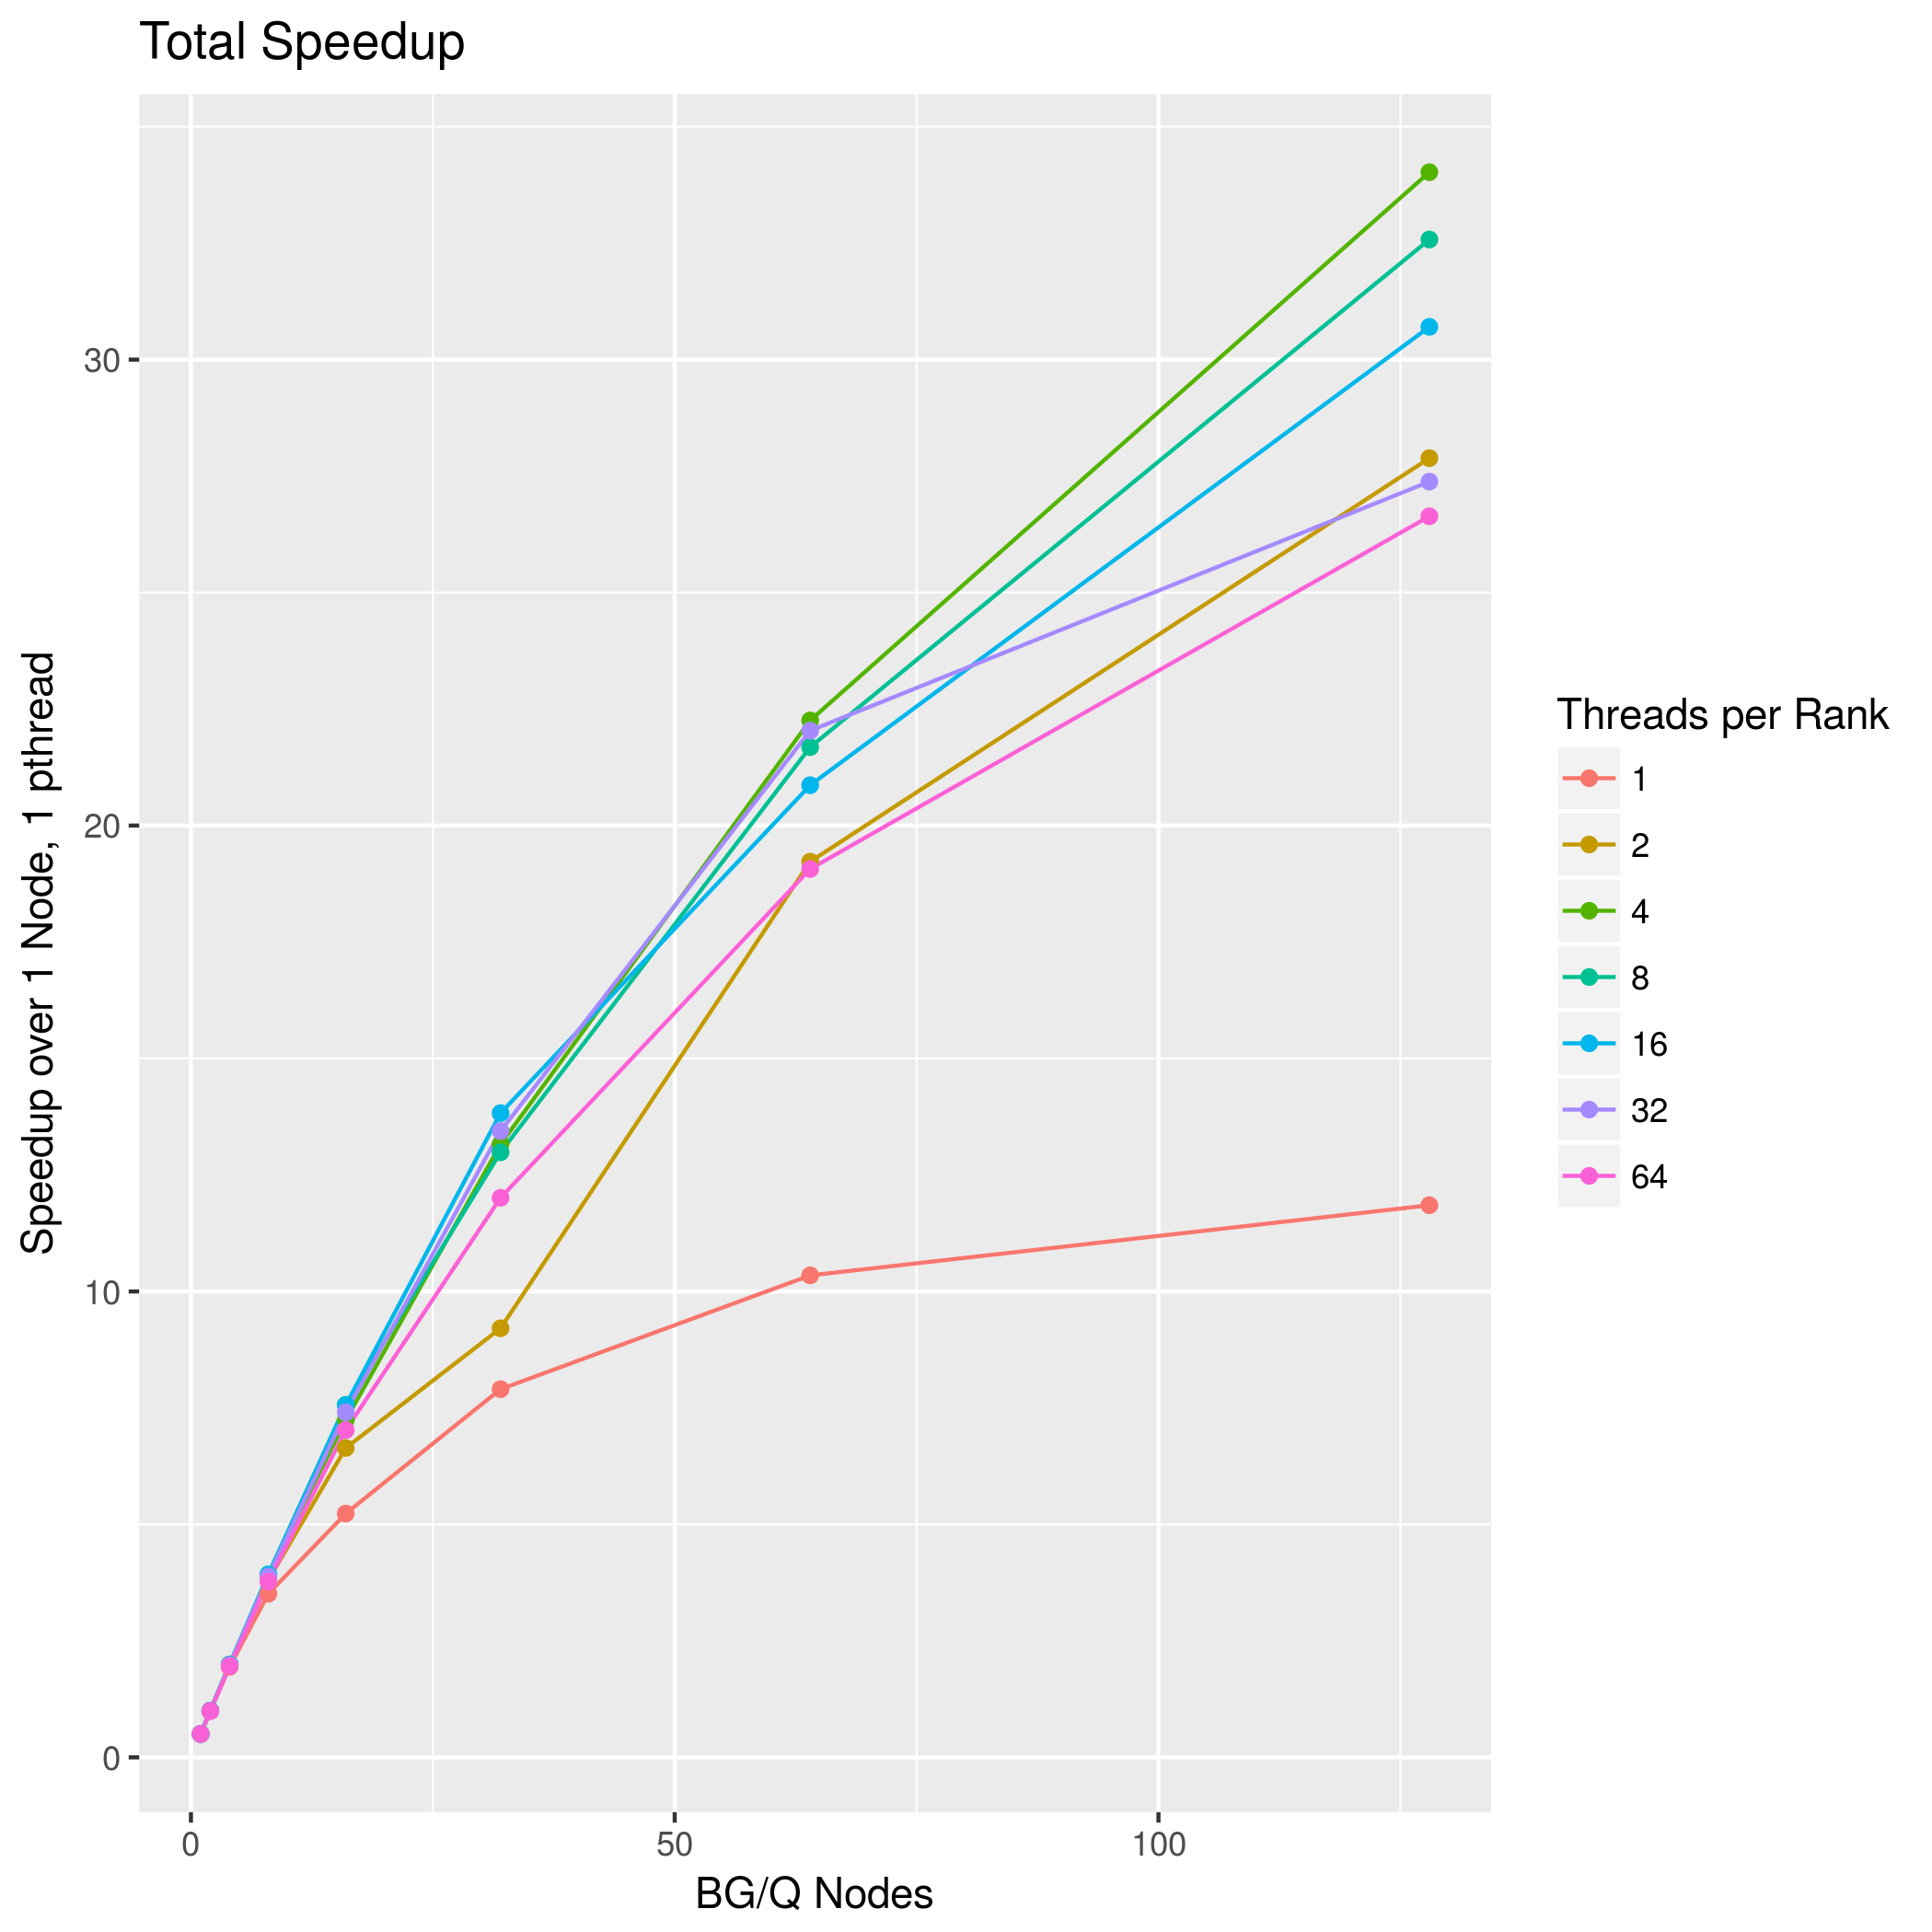
\includegraphics[width=\linewidth]{total_speedup.pdf}
  \caption{Speedup vs 64 ranks, 0 pthreads (1 BG/Q Node) time for 8192
    birds and 1000 iterations.\label{fig:totalspeedup}}
\end{figure}

The speedup relative to 64 MPI ranks and one pthread per rank (using
one BG/Q node) is shown in Figure \ref{fig:totalspeedup}. Our maximum
speedup was 67.518x which was achieved with 2048 MPI ranks and four
pthreads per rank. Much like Figure \ref{fig:total} the more extreme
thread per rank configurations, such as 1, 2, 32, and 64 pthreads per
rank perform much worse than the more balanced configurations.

\subsection*{Compute vs. Communication}

\begin{figure}[h!]
  \centering
  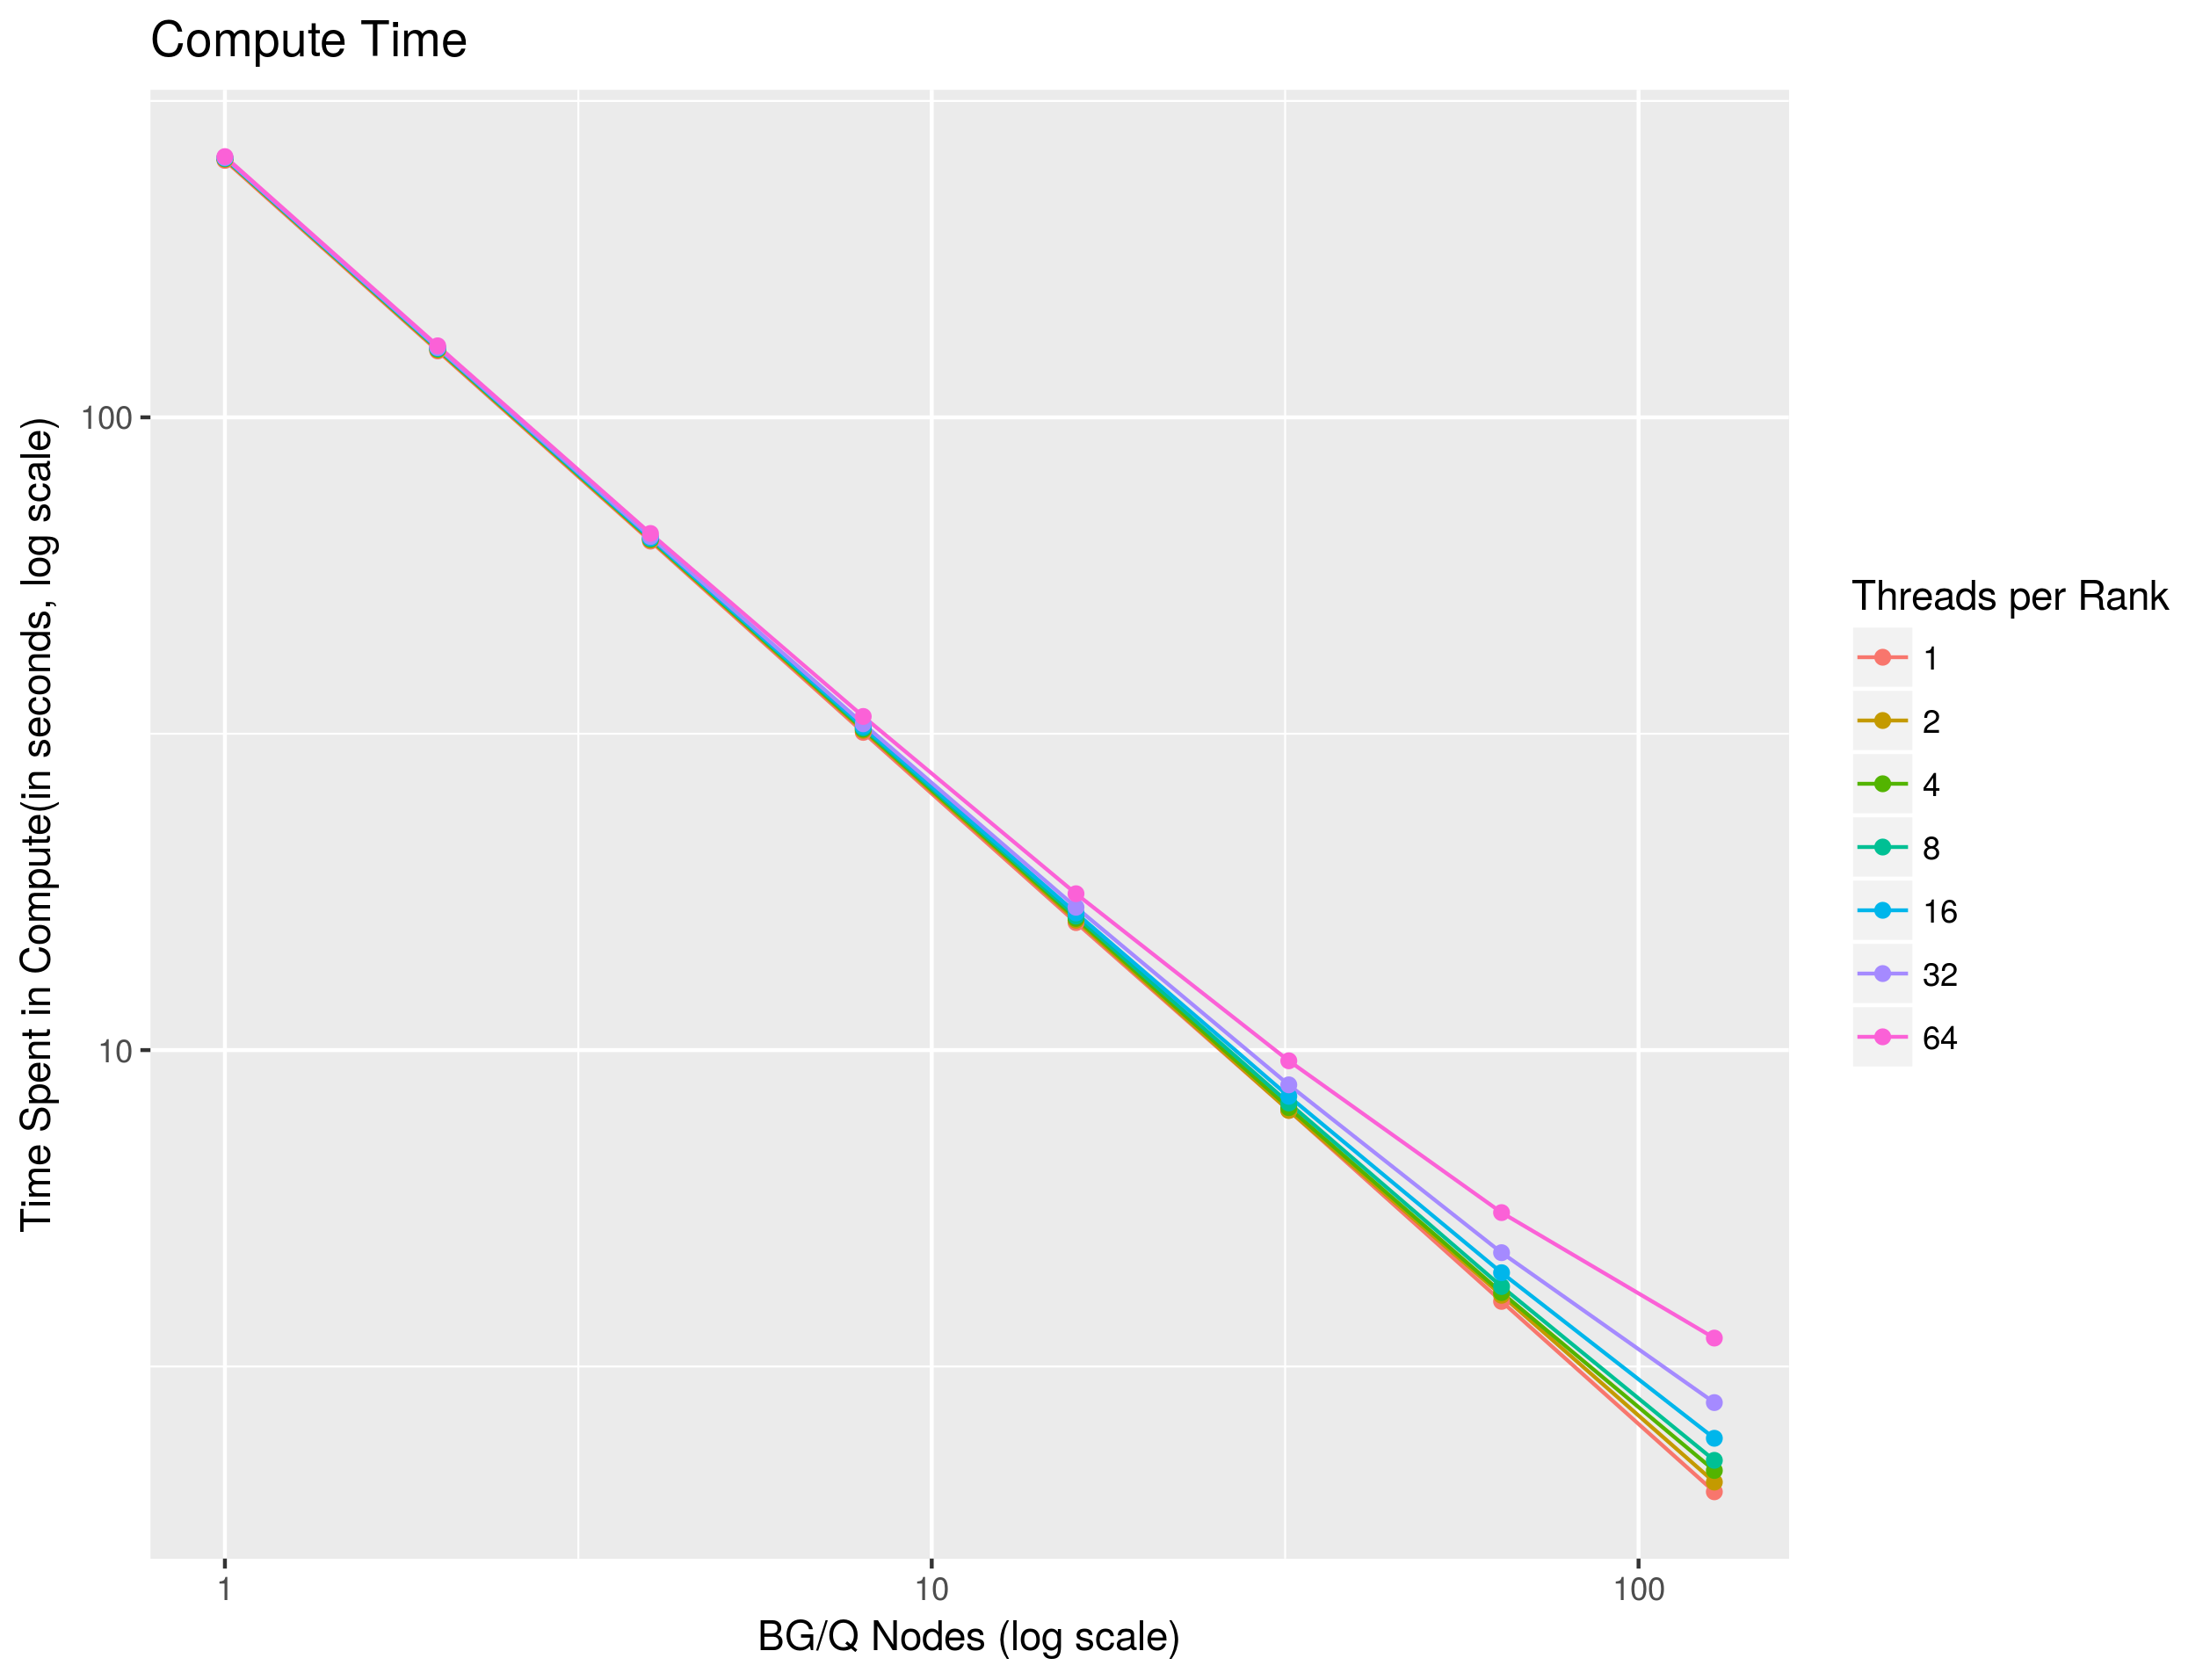
\includegraphics[width=\linewidth]{compute_time.pdf}
  \caption{Time spent computing bird positions and movements (8192
    birds and 1000 iterations).\label{fig:compute}}
\end{figure}

The compute time (Figure \ref{fig:compute}) initially resembles the
plot of the total execution time from Figure \ref{fig:total} for less
than 512 ranks and threads (or 8 compute nodes). However, as we
continue to scale up, we see that the lower thread per rank
configurations had better performance than the configurations with
more threads.

\begin{figure}[h!]
  \centering
  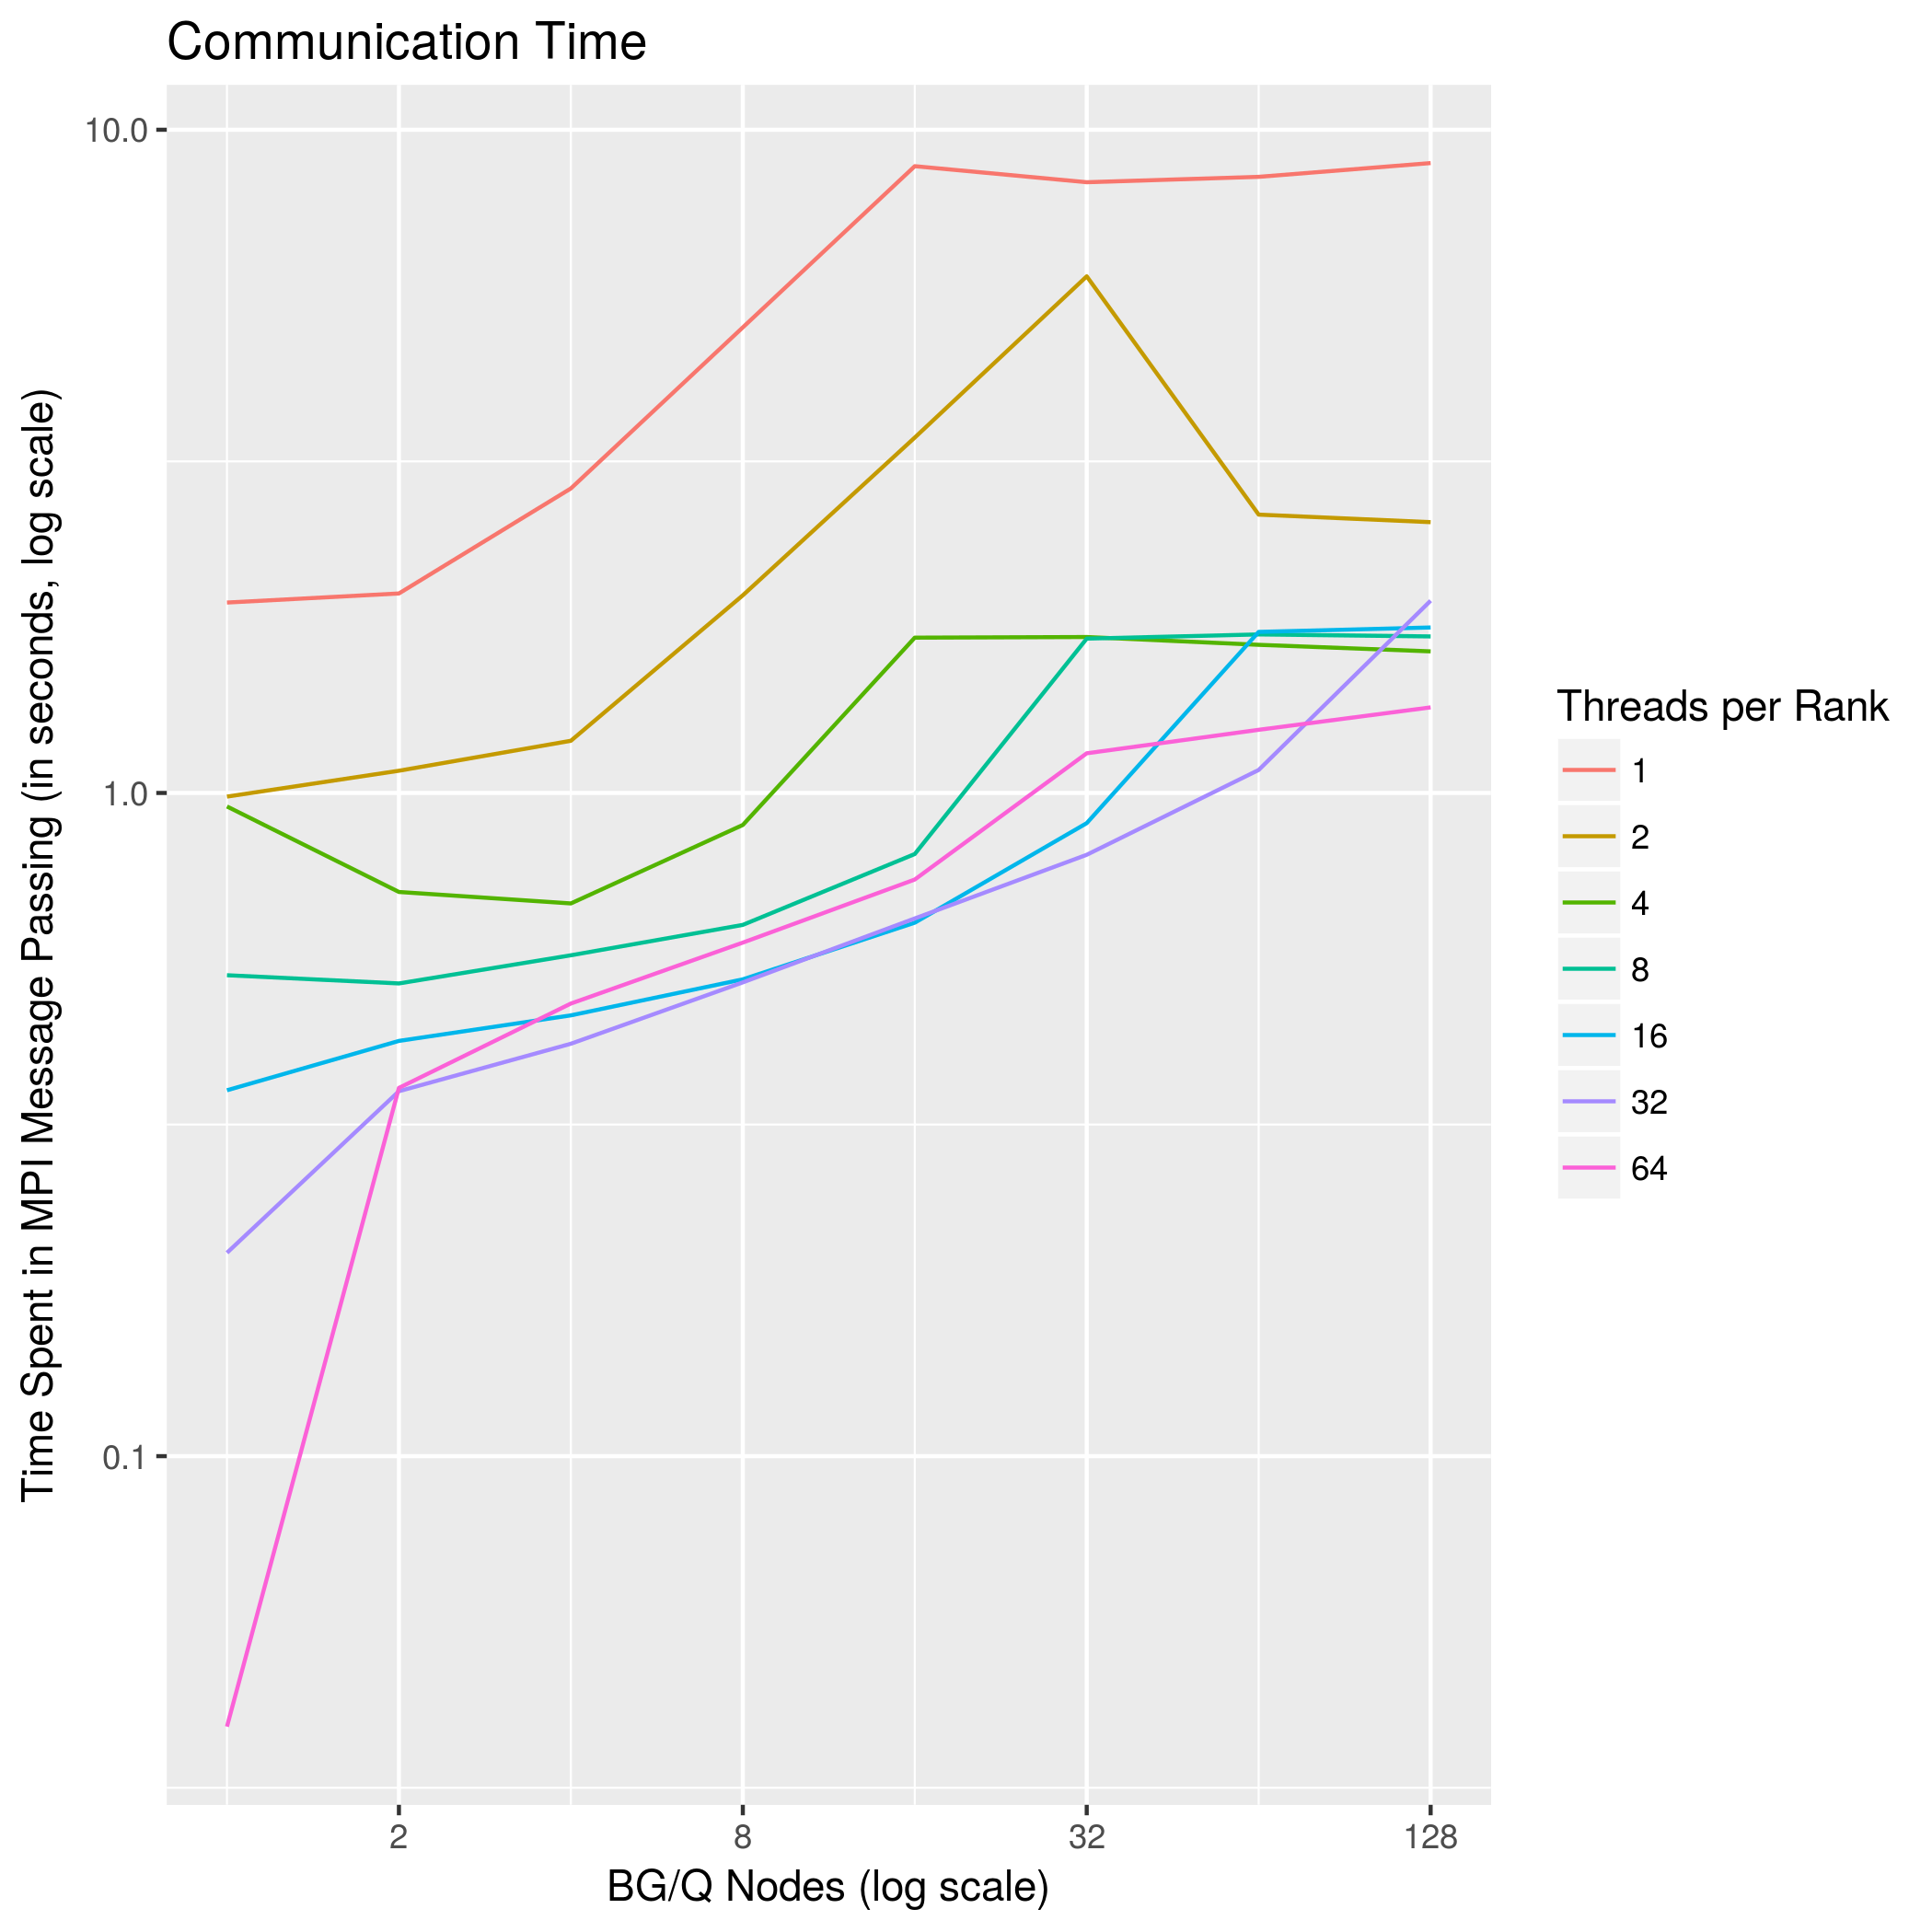
\includegraphics[width=\linewidth]{comm_time.pdf}
  \caption{Time spent doing MPI communications (8192 birds and 1000
    iterations).\label{fig:comm}}
\end{figure}

Overall, when using more threads per rank (and thus less MPI ranks)
the time spent in MPI communication functions decreases (Figure
\ref{fig:comm}). The total number of ranks and threads used together,
however, does not seem to have a significant impact on communication
time.

\begin{figure}[h!]
  \centering
  \includegraphics[width=\linewidth]{comm_percent.pdf}
  \caption{Percent of total time spent on MPI communication.\label{fig:commpercent}}
\end{figure}

Figure \ref{fig:commpercent}, which shows the percent of total
computation devoted to MPI message passing, gives another perspective
on the interaction of the communication and compute times. We see that
the proportion of time spent communicating very quickly increases as
the total number of ranks used increases, and that configurations with
fewer threads and more MPI ranks spend much more time on MPI
communications.

\subsection*{Multi-Threading}
\FloatBarrier
\begin{figure}[h!]
  \centering
  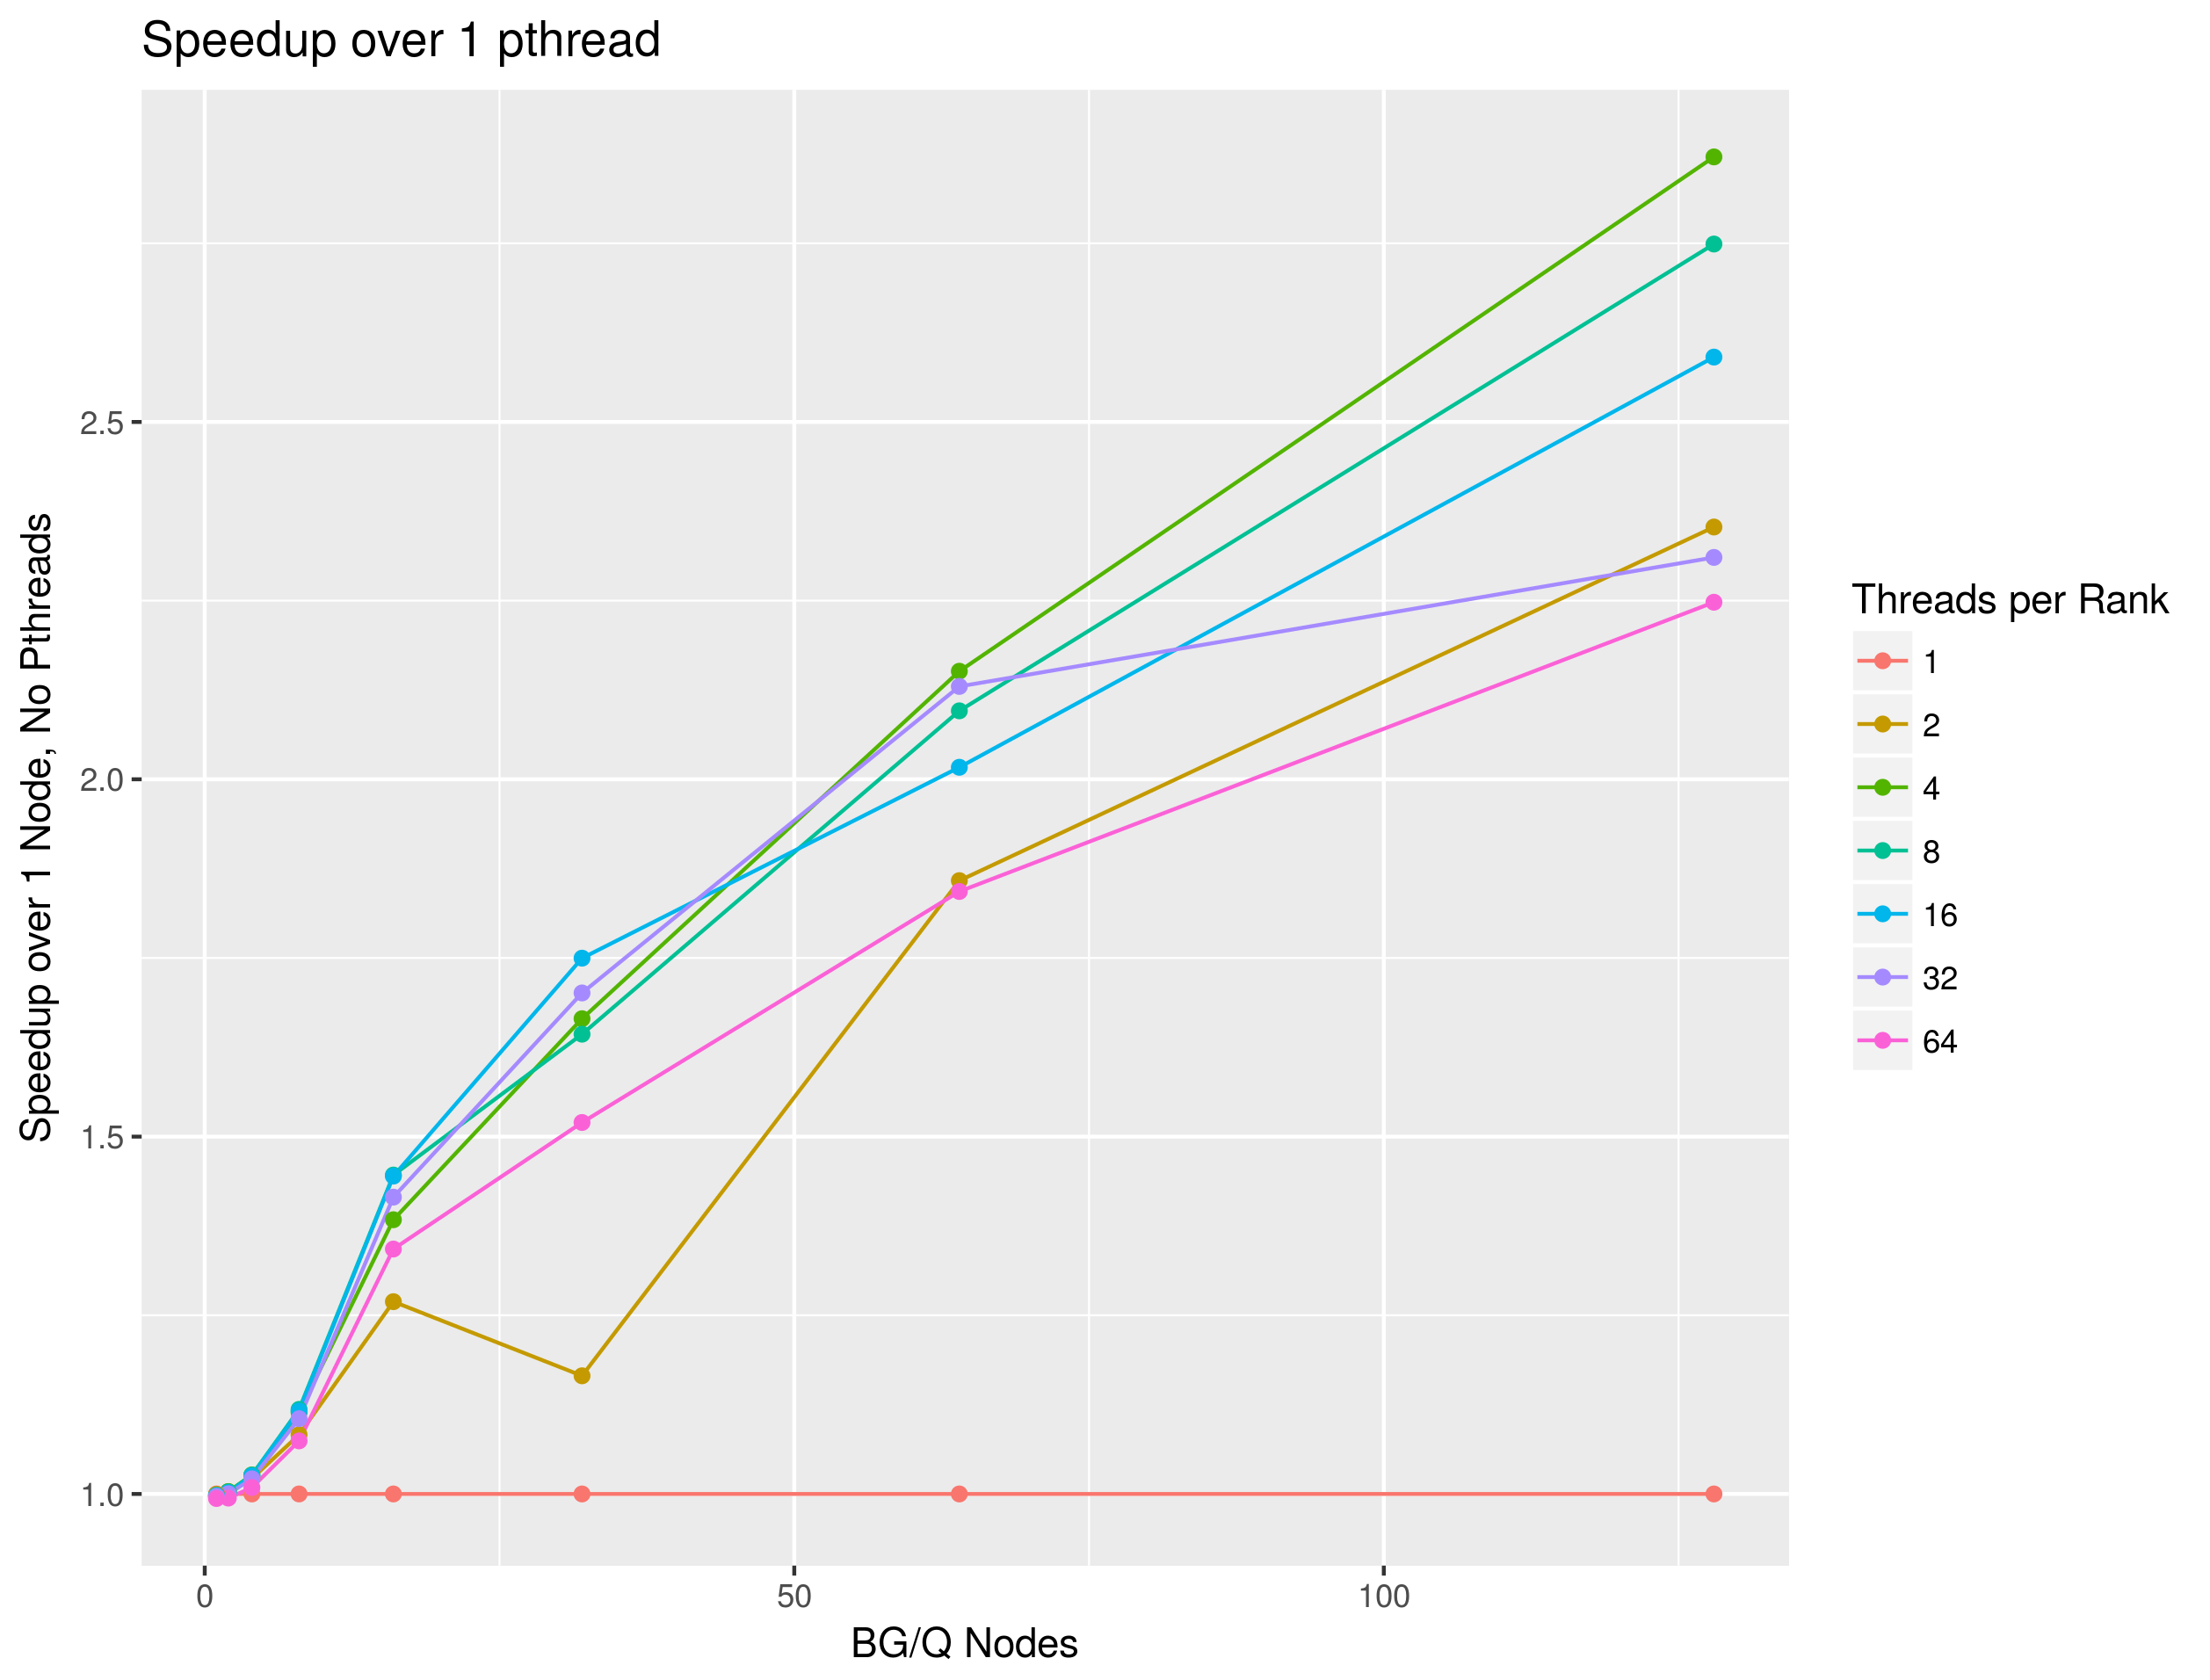
\includegraphics[width=\linewidth]{thread_speedup.pdf}
  \caption{Speedup vs using only 1 thread per rank (8192 birds and
    1000 iterations).\label{fig:threads}}
\end{figure}

Figure \ref{fig:threads} shows the total speedup over using a single
thread per rank.  Overall, the middle thread per rank configurations
(4, 8, and 16 threads) performed the best, while the configurations
with many or few threads per rank did not perform as well.

\subsection*{Weak Scaling}
\FloatBarrier
\begin{figure}[h!]
  \centering
  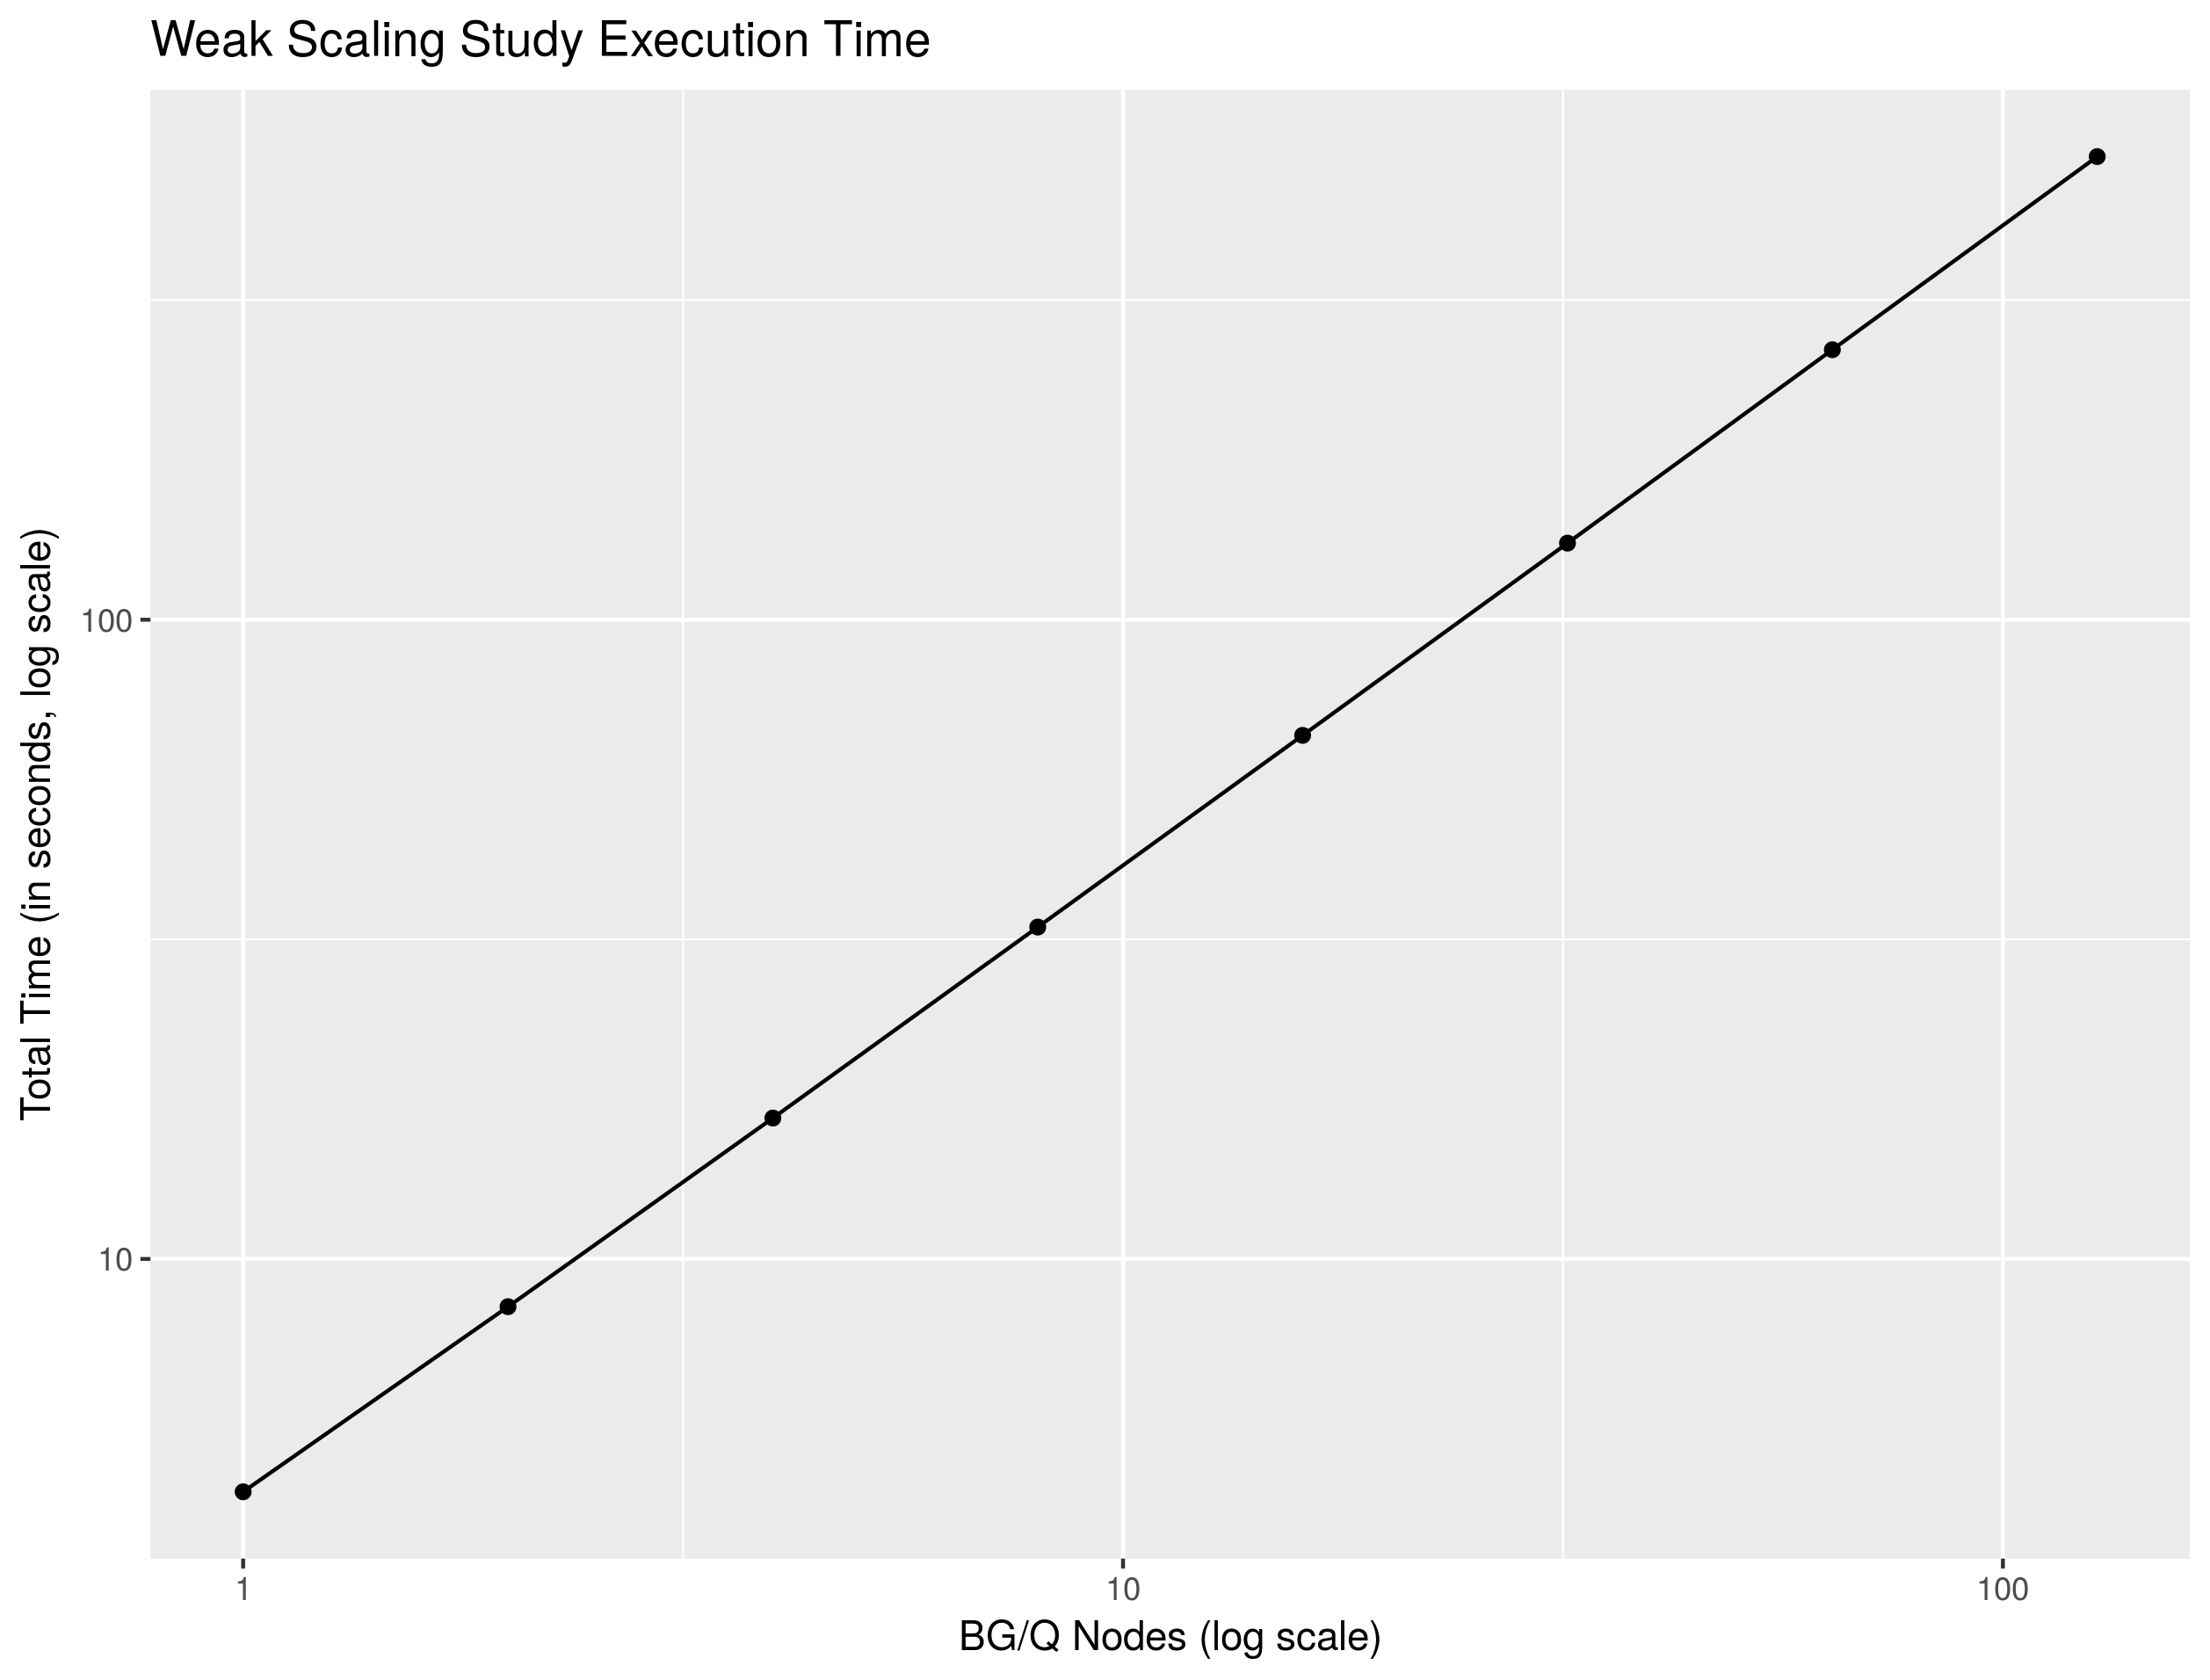
\includegraphics[width=\linewidth]{weakscaling.pdf}
  \caption{Execution time using 1024 birds/node, with 16 MPI
    ranks/node and 4 pthreads/MPI rank.\label{fig:weakscaling}}
\end{figure}

After our strong scaling study, we performed a weak scaling study by
running a simulation on 1, 2, 4, 8, 16, 32, 64, and 128 nodes for 1000
iterations using 1024 birds per node. Since our strong scaling study
revealed that using 4 pthreads per rank performed the best, we
proceded to use 16 MPI ranks and 4 pthreads per BG/Q compute node,
this means that each parallel thread was responsible for 16
birds. Figure \ref{fig:weakscaling} shows the total execution time
needed to run the simulation for each level of ranks and threads used.

\begin{figure}[h!]
  \centering
  \includegraphics[width=\linewidth]{eventspersec.pdf}
  \caption{Events per second using 1024 birds/node, with 16 MPI
    ranks/node and 4 pthreads/MPI rank.\label{fig:eventspersec}}
\end{figure}

We considered every bird movement and preceding computation to be a
single ``event''.  Figure \ref{fig:eventspersec} shows the number of
bird movement events that were computed per second for each level of
the weak scaling study.
